\documentclass[a4paper]{article}
% Some basic packages
\usepackage[utf8]{inputenc}
\usepackage[T1]{fontenc}
\usepackage{textcomp}
\usepackage[english]{babel}
\usepackage{url}
\usepackage{graphicx}
\usepackage{float}
\usepackage{booktabs}
\usepackage{enumitem}
\usepackage{tikz-cd}

\pdfminorversion=7

% Don't indent paragraphs, leave some space between them
\usepackage{parskip}

% Hide page number when page is empty
\usepackage{emptypage}
\usepackage{subcaption}
\usepackage{multicol}
\usepackage{xcolor}

% Math stuff
\usepackage{amsmath, amsfonts, mathtools, amsthm, amssymb}
\usepackage{mathrsfs}
\usepackage{cancel}
\usepackage{bm}
\newcommand\N{\ensuremath{\mathbb{N}}}
\newcommand\R{\ensuremath{\mathbb{R}}}
\newcommand\Z{\ensuremath{\mathbb{Z}}}
\renewcommand\O{\ensuremath{\emptyset}}
\newcommand\Q{\ensuremath{\mathbb{Q}}}
\newcommand\C{\ensuremath{\mathbb{C}}}

\usepackage{systeme}

\let\svlim\lim\def\lim{\svlim\limits}

\let\implies\Rightarrow
\let\impliedby\Leftarrow
\let\iff\Leftrightarrow
\let\epsilon\varepsilon

\usepackage{stmaryrd}
\newcommand\contra{\scalebox{1.5}{$\lightning$}}

\definecolor{correct}{HTML}{009900}
\newcommand\correct[2]{\ensuremath{\:}{\color{red}{#1}}\ensuremath{\to }{\color{correct}{#2}}\ensuremath{\:}}
\newcommand\green[1]{{\color{correct}{#1}}}

\newcommand\hr{
    \noindent\rule[0.5ex]{\linewidth}{0.5pt}
}

\newcommand\hide[1]{}

\usepackage{siunitx}
\sisetup{locale = US}

\usepackage{mdframed}
\mdfsetup{skipabove=1em,skipbelow=0em}
\theoremstyle{definition}
\newmdtheoremenv[nobreak=true]{definition}{Definition}
\newmdtheoremenv[nobreak=true]{property}{Property}
\newmdtheoremenv[nobreak=true]{corollary}{Corollary}
\newmdtheoremenv[nobreak=true]{theorem}{Theorem}
\newmdtheoremenv[nobreak=true]{lemma}{Lemma}
\newmdtheoremenv[nobreak=true]{proposition}{Proposition}

\newtheorem*{example}{Example}
\newtheorem*{notation}{Notation}
\newtheorem*{remark}{Remark}
\newtheorem*{note}{Note}
\newtheorem*{problem}{Problem}
\newtheorem*{observe}{Observe}
\newtheorem*{intuition}{Intuition}
% ... (add other unnumbered theorem-like environments as per your requirement)

\usepackage{etoolbox}
\AtEndEnvironment{example}{\null\hfill$\diamond$}%
% ... (add other environments to end with a diamond if required)

\makeatletter
\def\thm@space@setup{%
  \thm@preskip=\parskip \thm@postskip=0pt
}

\newcommand{\exercise}[1]{%
    \def\@exercise{#1}%
    \subsection*{Exercise #1}
}

\newcommand{\subexercise}[1]{%
    \subsubsection*{Exercise \@exercise.#1}
}

\usepackage{xifthen}
\def\testdateparts#1{\dateparts#1\relax}
\def\dateparts#1 #2 #3 #4 #5\relax{
    \marginpar{\small\textsf{\mbox{#1 #2 #3 #5}}}
}

\def\@lecture{}%
\newcommand{\lecture}[3]{
    \ifthenelse{\isempty{#3}}{%
        \def\@lecture{Lecture #1}%
    }{%
        \def\@lecture{Lecture #1: #3}%
    }%
    \subsection*{\@lecture}
    \marginpar{\small\textsf{\mbox{#2}}}
}

\usepackage{fancyhdr}
\pagestyle{fancy}

\fancyhead[RO,LE]{\@lecture}
\fancyfoot[RO,LE]{\thepage}
\fancyfoot[C]{\leftmark}

\makeatother

\usepackage{todonotes}
\usepackage{tcolorbox}

\tcbuselibrary{breakable}

\newenvironment{correction}{\begin{tcolorbox}[
    arc=0mm,
    colback=white,
    colframe=green!60!black,
    title=Remark,
    fonttitle=\sffamily,
    breakable
]}{\end{tcolorbox}}

\newenvironment{notebox}[1]{\begin{tcolorbox}[
    arc=0mm,
    colback=white,
    colframe=white!60!black,
    title=#1,
    fonttitle=\sffamily,
    breakable
]}{\end{tcolorbox}}

\usepackage{import}
\usepackage{pdfpages}
\usepackage{transparent}
\newcommand{\incfig}[1]{%
    \def\svgwidth{\columnwidth}
    \import{./figures/}{#1.pdf_tex}
}

\pdfsuppresswarningpagegroup=1

\author{Mika Bohinen}

\usepackage{istgame}
\title{Computational Game Theory \\ Sheet 4 \\
Class Tutor: Mr C. Wang}
\begin{document}
\maketitle
\begin{exercise}{1}
\end{exercise}
\begin{enumerate}[label=(\alph*)]
  \item Given the game matrix, the expressions for the expected utilities are as follows:

    \textbf{For} \(\pi_1(p, L)\):
    \begin{align*}
      \pi_1(p, L) &= 2 \cdot p + (-1) \cdot (1-p) \\
                  &= 2p - 1 + p \\
                  &= 3p - 1
    \end{align*}

    \textbf{For} \(\pi_1(p, R)\):
    \begin{align*}
      \pi_1(p, R) &= (-3) \cdot p + 1 \cdot (1-p) \\
                  &= -3p + 1 - p \\
                  &= -4p + 1
    \end{align*}

    \textbf{For} \(\pi_1(T, q)\):
    \begin{align*}
      \pi_1(T, q) &= 2 \cdot q + (-3) \cdot (1-q) \\
                  &= 2q - 3 + 3q \\
                  &= 5q - 3
    \end{align*}

    \textbf{For} \(\pi_1(B, q)\):
    \begin{align*}
      \pi_1(B, q) &= (-1) \cdot q + 1 \cdot (1-q) \\
                  &= -q + 1 - q \\
                  &= 1 - 2q
    \end{align*}

  \item

    In this exercise, we consider the functions $\pi_1(p, L) = 3p - 1$ and $\pi_1(p, R) = -4p + 1$. The plot (see Figure \ref{fig:1b}) illustrates these two functions and the minimum of these functions across the range of $p$ from 0 to 1.

    \begin{figure}[ht]
      \centering
      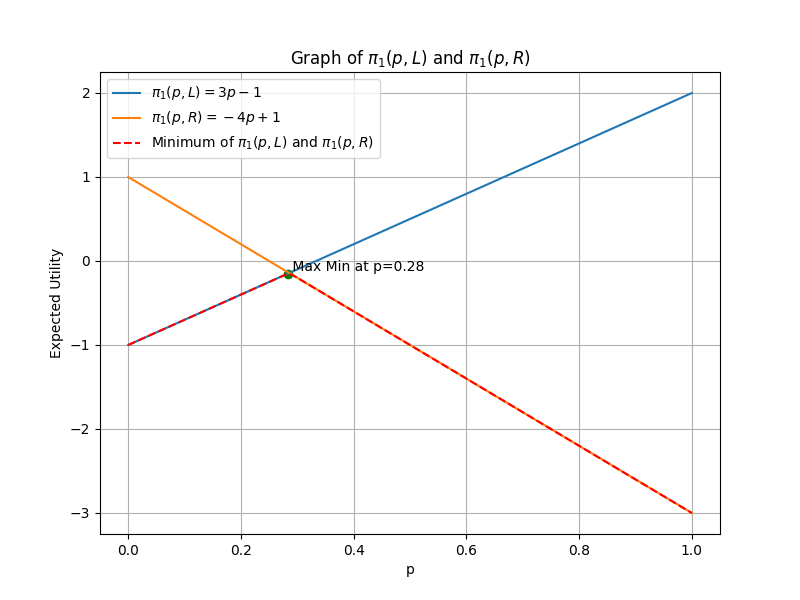
\includegraphics[width=0.8\textwidth]{./figures/tut4_1b.png}
      \caption{Plot of $\pi_1(p, L)$ and $\pi_1(p, R)$ showing the minimum of these functions.}
      \label{fig:1b}
    \end{figure}

    To find the maximum of the minimum of these functions, we need to determine the point at which $\pi_1(p, L)$ and $\pi_1(p, R)$ intersect. Setting $\pi_1(p, L) = \pi_1(p, R)$, we have:

    \begin{align*}
      3p - 1 &= -4p + 1 \\
      7p &= 2 \\
      p &= \frac{2}{7}
    \end{align*}

    At $p = \frac{2}{7}$, both functions have the same value, and this is the point at which the minimum of these functions takes its maximum value. Substituting $p = \frac{2}{7}$ into either function gives us the maximum of the minimum value:

    \begin{align*}
      \pi_1\left(\frac{2}{7}, L\right) = 3\left(\frac{2}{7}\right) - 1 = -\frac{1}{7}
    \end{align*}

    Thus, the maximum value of the minimum of $\pi_1(p, L)$ and $\pi_1(p, R)$ is $-\frac{1}{7}$, occurring at $p = \frac{2}{7}$. This point is crucial in analyzing the zero-sum game as it suggests the optimal mixed strategy for player 1 in this scenario.

  \item
    This part of the exercise involves analyzing the functions $\pi_1(T, q) = 5q - 3$ and $\pi_1(B, q) = 1 - 2q$. The plot (refer to Figure \ref{fig:1c}) depicts these functions and the maximum of these functions for the range of $q$ from 0 to 1.

    \begin{figure}[ht]
      \centering
      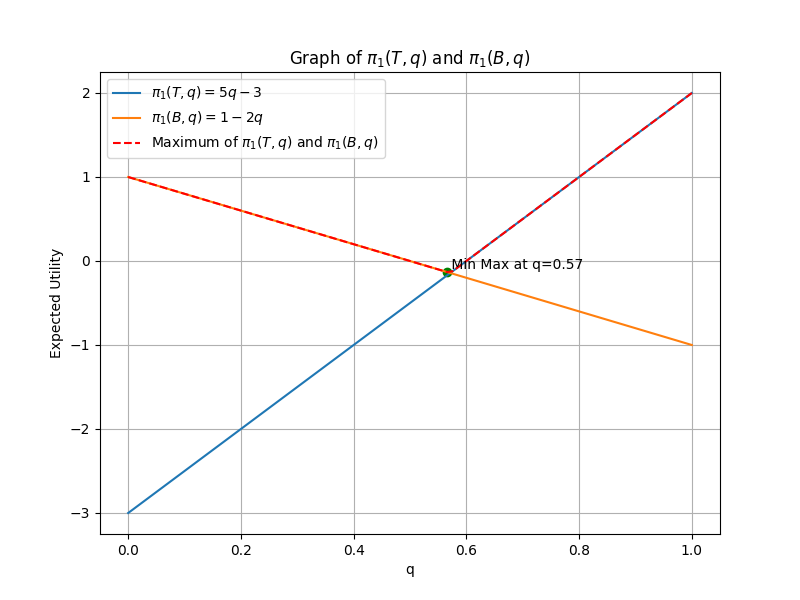
\includegraphics[width=0.8\textwidth]{figures/tut4_1c.png}
      \caption{Plot of $\pi_1(T, q)$ and $\pi_1(B, q)$ showing the maximum of these functions.}
      \label{fig:1c}
    \end{figure}

    To find the minimum of the maximum of these functions, we equate $\pi_1(T, q)$ and $\pi_1(B, q)$:

    \begin{align*}
      5q - 3 &= 1 - 2q \\
      7q &= 4 \\
      q &= \frac{4}{7}
    \end{align*}

    At $q = \frac{4}{7}$, the functions intersect, indicating the point where the maximum of these functions takes its minimum value. Substituting $q = \frac{4}{7}$ into either function yields:

    \begin{align*}
      \pi_1\left(T, \frac{4}{7}\right) &= 5 \cdot \frac{4}{7} - 3 = \frac{5}{7} - 3 = -\frac{16}{7}
    \end{align*}

    Thus, the minimum value of the maximum of $\pi_1(T, q)$ and $\pi_1(B, q)$ is $-\frac{16}{7}$, occurring at $q = \frac{4}{7}$. This point is significant for determining the optimal strategy for player 2 in this game, indicating the mixed strategy that minimizes the maximum payoff player 1 can achieve.


  \item
    The analysis of the graphs in Exercises 1 (b) and (c) provides crucial insights into the zero-sum game described.

    \textbf{Significance of the Graphs:}
    \begin{itemize}
      \item In Exercise 1 (b), the plot of $\pi_1(p, L)$ and $\pi_1(p, R)$, and particularly the maximum of their minimum, indicates the best strategy for player 1. At $p = \frac{2}{7}$, player 1 minimizes their maximum loss, which is a key strategy in zero-sum games.
      \item Similarly, in Exercise 1 (c), the plot of $\pi_1(T, q)$ and $\pi_1(B, q)$, and the minimum of their maximum, demonstrates the best strategy for player 2. The point $q = \frac{4}{7}$ indicates where player 2 can minimize the maximum gain of player 1.
    \end{itemize}

    \textbf{Optimal Strategies and Equilibrium Outcome:}
    \begin{itemize}
      \item The optimal strategy for player 1 is to play a mixed strategy with $p = \frac{2}{7}$, which means choosing strategy T with probability $\frac{2}{7}$ and strategy B with probability $\frac{5}{7}$.
      \item For player 2, the optimal strategy is a mixed strategy with $q = \frac{4}{7}$, choosing strategy L with probability $\frac{4}{7}$ and strategy R with probability $\frac{3}{7}$.
      \item These strategies lead to an equilibrium outcome where neither player can unilaterally change their strategy to improve their expected payoff.
    \end{itemize}

    \textbf{Value of the Game:}
    \begin{itemize}
      \item The value of the game is determined at the equilibrium point. Substituting $p = \frac{2}{7}$ and $q = \frac{4}{7}$ into either $\pi_1(p, L)$ or $\pi_1(T, q)$, we find that the value of the game is $-\frac{1}{7}$.
      \item This value represents the expected payoff for player 1 (and the expected loss for player 2) when both players play their optimal strategies.
    \end{itemize}

    In conclusion, the analysis of these graphs in a zero-sum game context reveals the optimal mixed strategies for both players and the equilibrium outcome of the game. The game's value indicates the payoff one player can expect to gain, which is symmetrically the loss the other player can expect, under these optimal strategies.
\end{enumerate}
\end{document}
